\begin{frame}[allowframebreaks]{Clases}\vspace{0pt}

Las clases son \textit{estructuras} o algoritmos que permiten dividir un concepto complejo en conceptos simples que pueden ser tanto \underline{generales} como \underline{detallados}. Para el caso del semillero, podríamos pensar en algo como esto:

\begin{figure}
	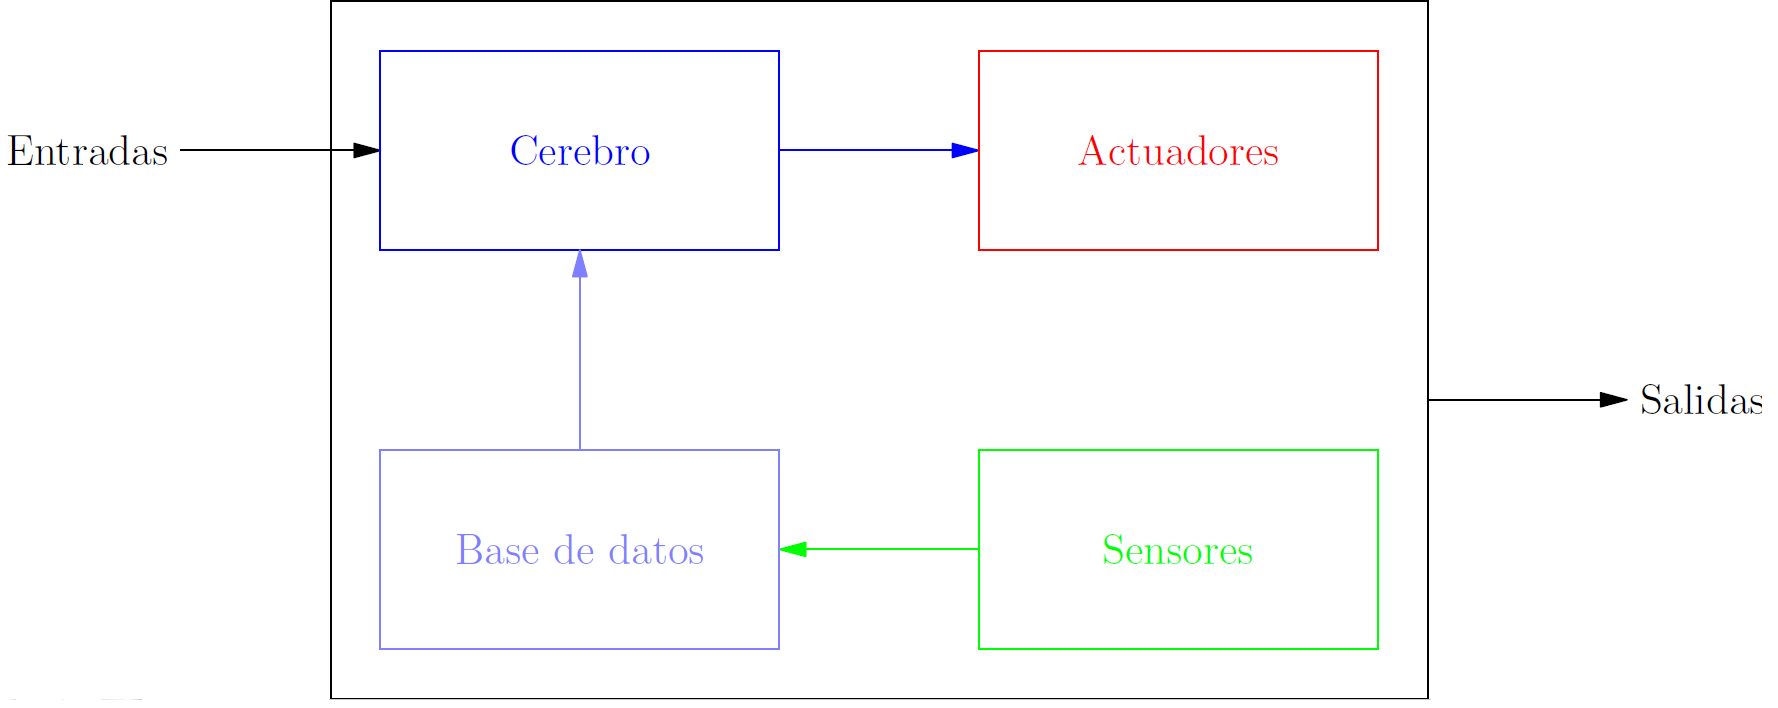
\includegraphics[scale=0.35]{Images/Esquema/Esquema.PNG}
\end{figure}

\vspace{30pt}

Las \textbf{entradas} del sistema son:

\begin{itemize}
	\item Tipo de cultivo.
	\item Ubicación de plantas.
	\item Fecha de desarrollo.
\end{itemize}

Las \textbf{salidas} son:

\begin{itemize}
	\item Cantidad de producto.
	\item Datos recolectados durante el desarrollo.
\end{itemize}

\end{frame}